The kinematic vertex fit of the tag-$B$ meson candidate (see \Cref{sec:event_reconstruction}) provides $x$, $y$ and $z$ coordinates of the decay.
True $B$ meson candidates should have successful fits, consistent with a decay near the collision point.

Furthermore, all other tracks, originating from particles that were not used in the reconstruction of the tag-$B$ meson have another vertex fit performed.
This gives another set of vertex variables, which is checked for kinematic consistency with the decay originating near the interaction point.
This fitted $B$ meson candidate is denoted as $B_{\mathrm{ROE}}$ and used only for continuum suppression.
In this analysis the following 19 observables are tested:
\begin{itemize}
    \item $x$, $y$ and $z$ are tag-$B$ vertex coordinate and their uncertainty distributions;
    \item $\chi_V^2$ of the tag-$B$ meson vertex fit;
    \item $x_{B_{\mathrm{ROE}}}$,$y_{B_{\mathrm{ROE}}}$,$z_{B_{\mathrm{ROE}}}$ and their uncertainty distributions;
    \item $B_{\mathrm{ROE}}$ vertex $p$-value;
    \item $\chi^2_{V}$: $B_{\mathrm{ROE}}$ vertex $\chi^2$ value;
    \item $\chi^2_{B_{\mathrm{ROE}};\mathrm{IP}}$: $B_{\mathrm{ROE}}$ vertex $\chi^2$ value of the interaction point component;
    \item $\Delta \tau$: proper decay time difference between tag-$B$ meson and $B_{\mathrm{ROE}}$;
    \item $\Delta z$: difference of decay vertex $z$ components between tag-$B$ meson and $B_{\mathrm{ROE}}$;
    \item $\Delta z_B$: difference of decay vertex $z$ components between tag-$B$ meson and $B_{\mathrm{ROE}}$ in the boost direction.
\end{itemize}

The results for \textbf{Test~1} are shown in \Cref{fig:Btag_x,fig:Btag_y,fig:Btag_z,fig:Btag_x_uncertainty,fig:Btag_y_uncertainty,fig:Btag_z_uncertainty,fig:Btag_chiProb,fig:Btag_TagVx,fig:Btag_TagVy,fig:Btag_TagVz,fig:Btag_TagVxErr,fig:Btag_TagVyErr,fig:Btag_TagVzErr,fig:Btag_TagVChi2,fig:Btag_TagVChi2IP,fig:Btag_TagVpVal,fig:Btag_DeltaT,fig:Btag_DeltaZ,fig:Btag_DeltaBoost}.
Most of these features show no correlation to \EB or \Estar, as the vertex requirement is a purely physical constraint.
The $\chi^2$ of tag-$B$ meson is manually excluded to avoid a bias towards selected \FEI modes.

\begin{figure}[htbp!]
    \centering
    \subcaptionbox{\label{fig:Btag_x}}{
        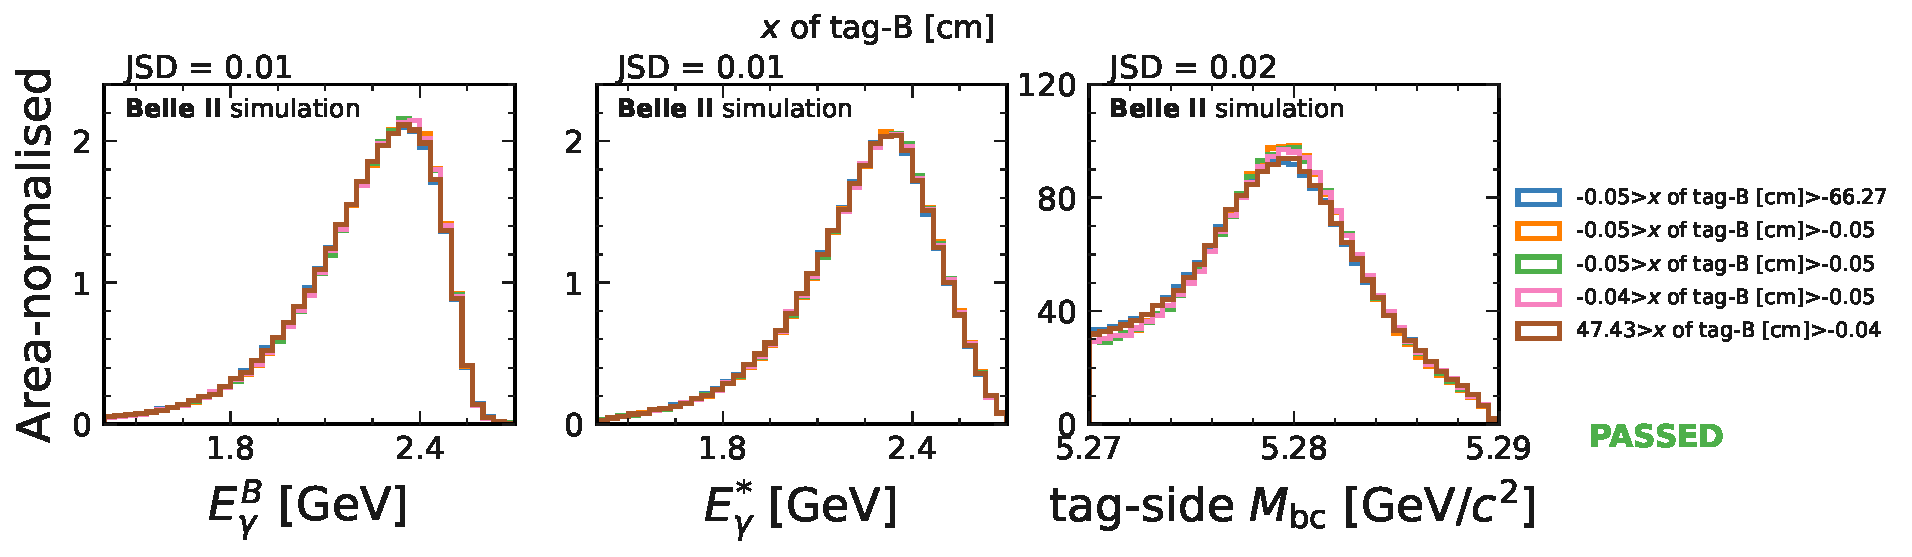
\includegraphics[width=0.95\textwidth]{figures/appendices/continuum_suppression_features/vertex_features/Btag_x_bias_tested.pdf}
    }
    \subcaptionbox{\label{fig:Btag_y}}{
        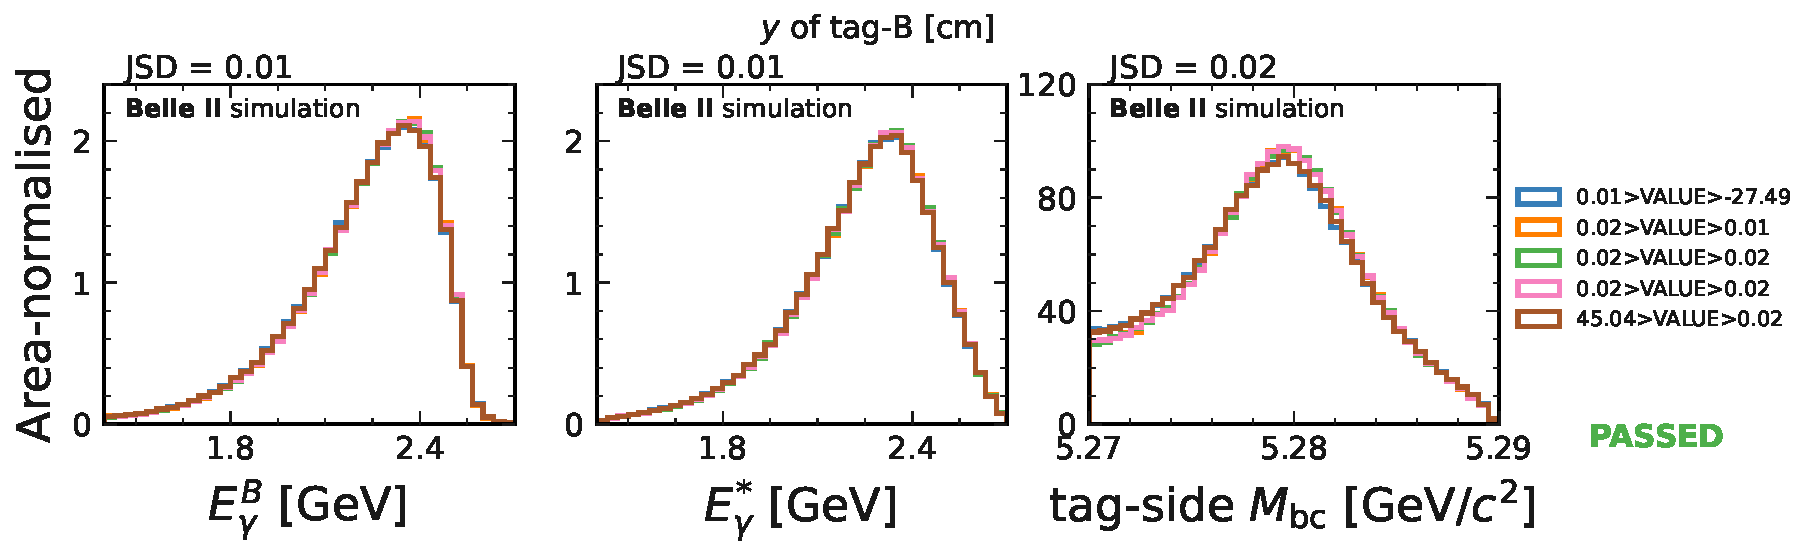
\includegraphics[width=0.95\textwidth]{figures/appendices/continuum_suppression_features/vertex_features/Btag_y_bias_tested.pdf}

    }
    \subcaptionbox{\label{fig:Btag_z}}{
        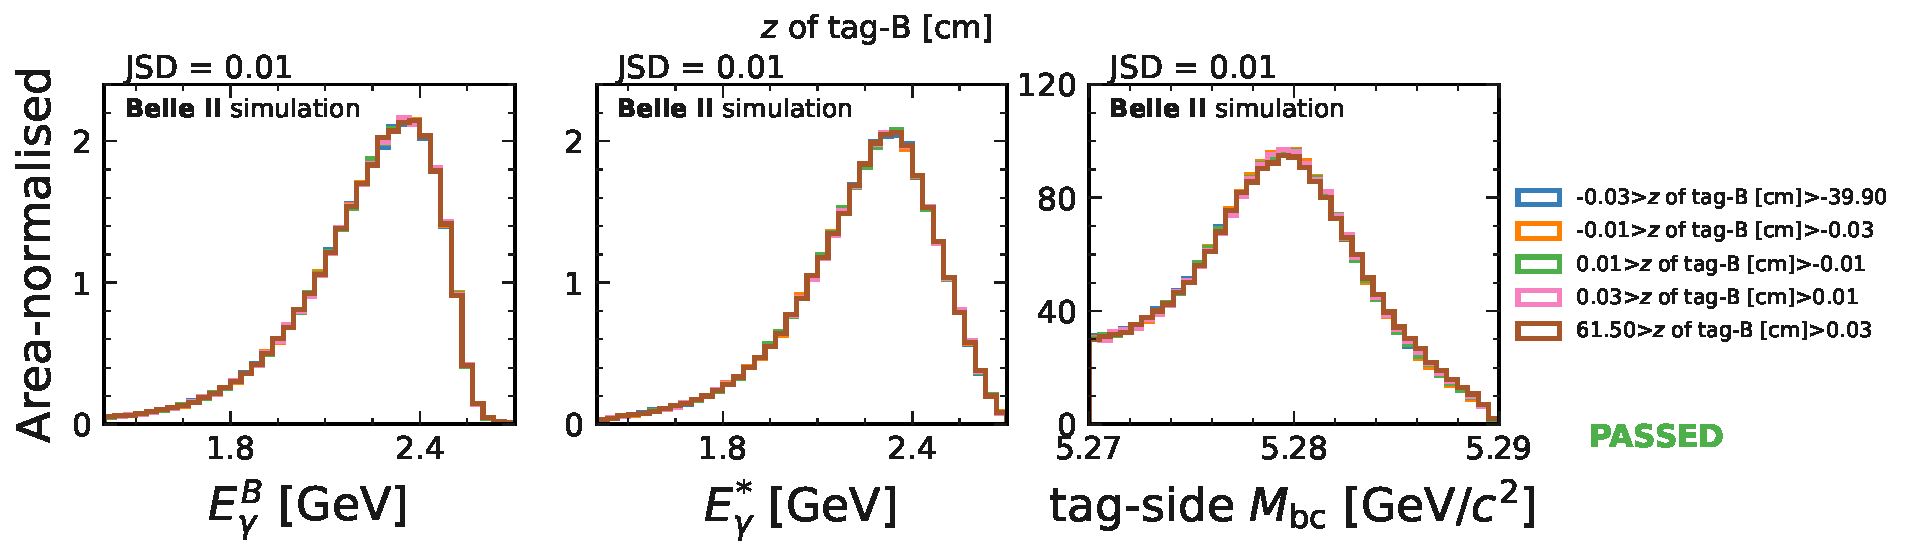
\includegraphics[width=0.95\textwidth]{figures/appendices/continuum_suppression_features/vertex_features/Btag_z_bias_tested.pdf}

    }
    \subcaptionbox{\label{fig:Btag_x_uncertainty}}{
        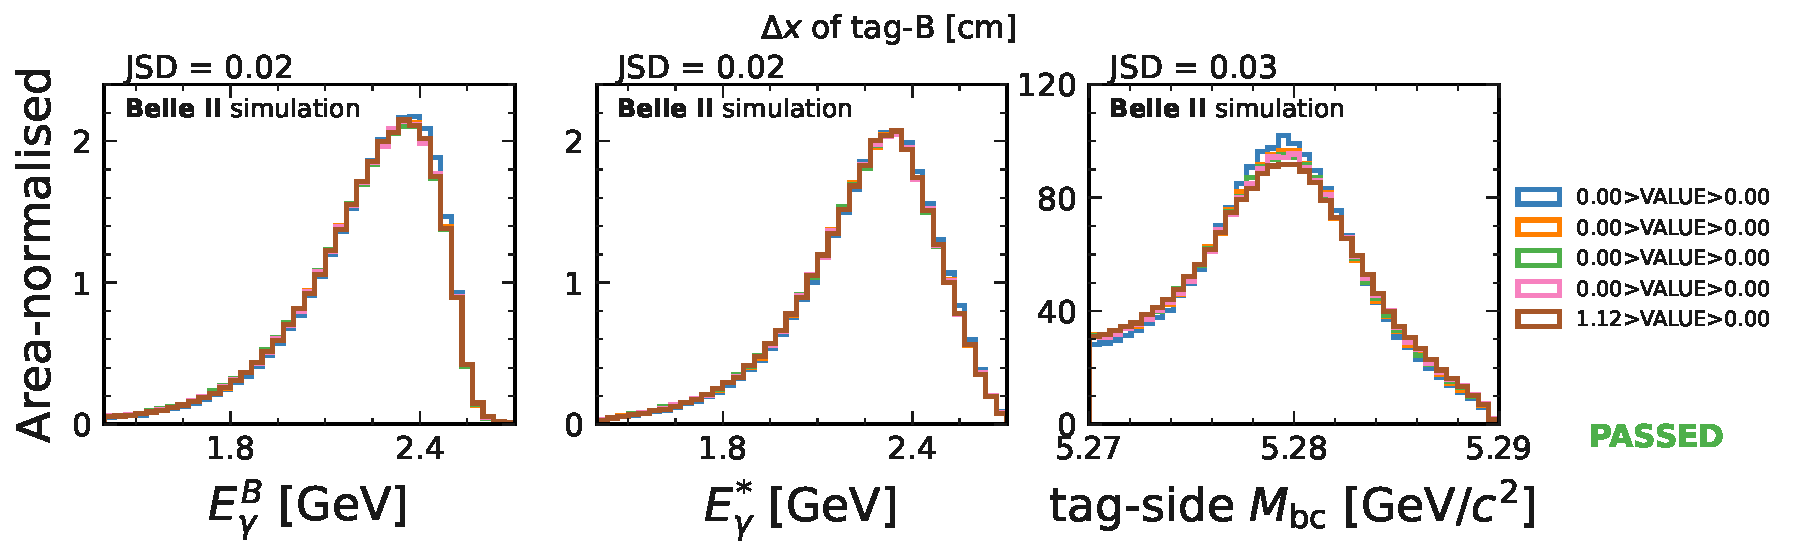
\includegraphics[width=0.95\textwidth]{figures/appendices/continuum_suppression_features/vertex_features/Btag_x_uncertainty_bias_tested.pdf}

    }
\end{figure}
\begin{figure}[htbp!]
    \centering
    \ContinuedFloat
    \subcaptionbox{\label{fig:Btag_y_uncertainty}}{
        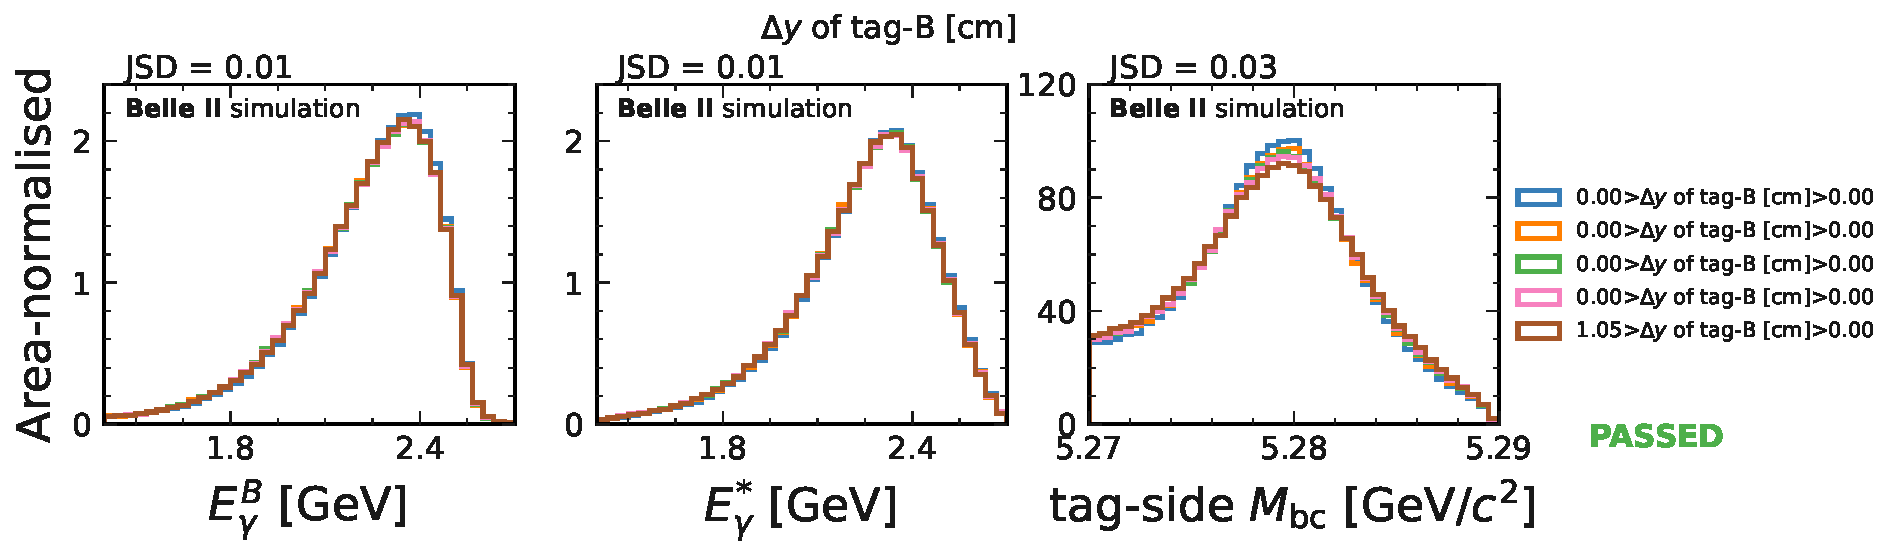
\includegraphics[width=0.95\textwidth]{figures/appendices/continuum_suppression_features/vertex_features/Btag_y_uncertainty_bias_tested.pdf}

    }
    \subcaptionbox{\label{fig:Btag_z_uncertainty}}{
        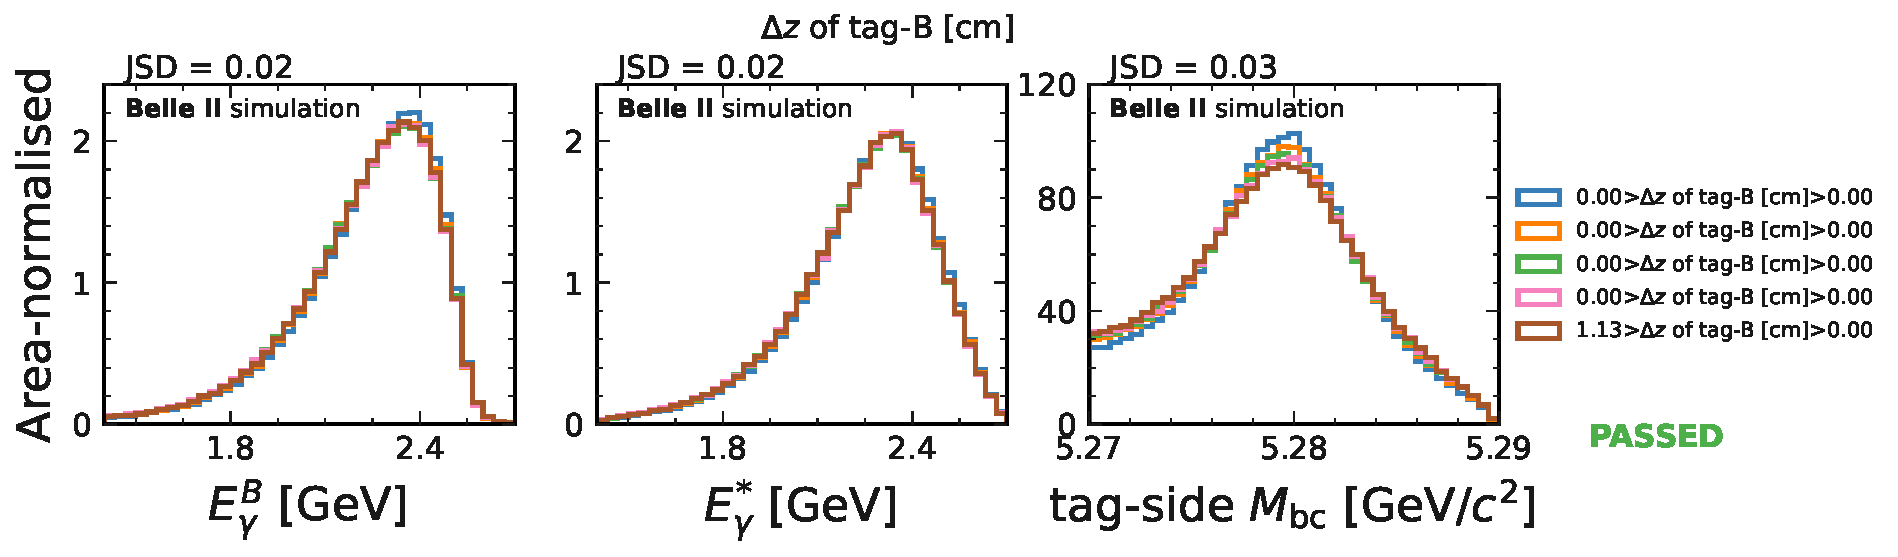
\includegraphics[width=0.95\textwidth]{figures/appendices/continuum_suppression_features/vertex_features/Btag_z_uncertainty_bias_tested.pdf}

    }
    \subcaptionbox{\label{fig:Btag_chiProb}}{
        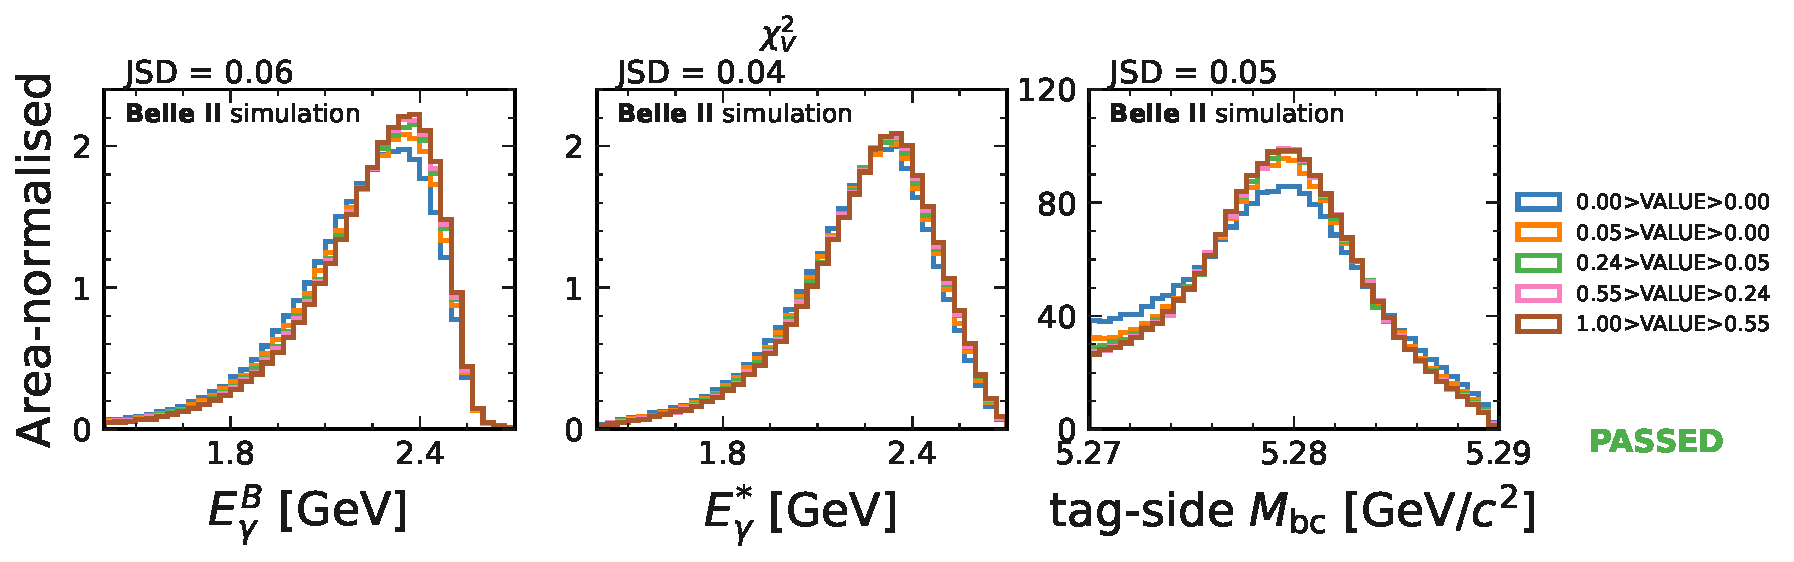
\includegraphics[width=0.95\textwidth]{figures/appendices/continuum_suppression_features/vertex_features/Btag_chiProb_bias_tested.pdf}

    }
    \subcaptionbox{\label{fig:Btag_TagVx}}{
        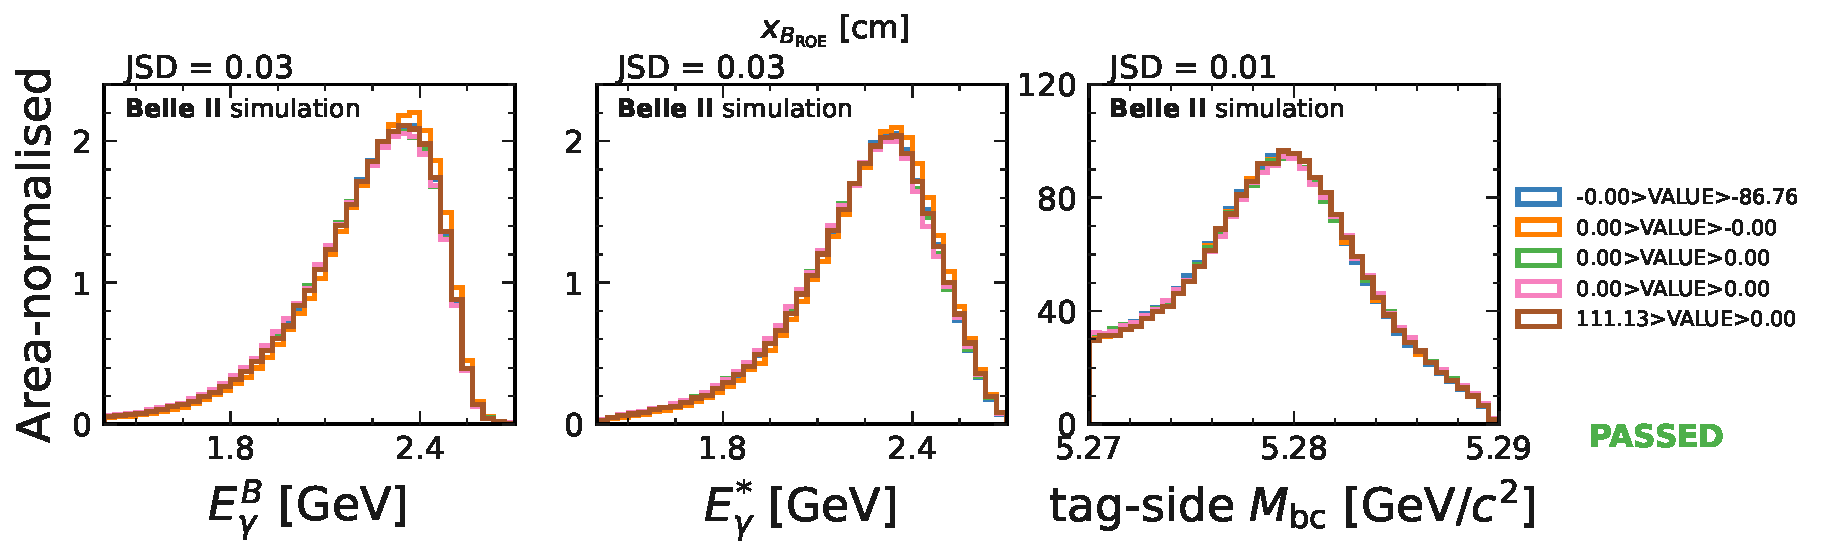
\includegraphics[width=0.95\textwidth]{figures/appendices/continuum_suppression_features/vertex_features/Btag_TagVxBeam_bias_tested.pdf}

    }
\end{figure}
\begin{figure}[htbp!]
    \centering
    \ContinuedFloat
    \subcaptionbox{\label{fig:Btag_TagVy}}{
        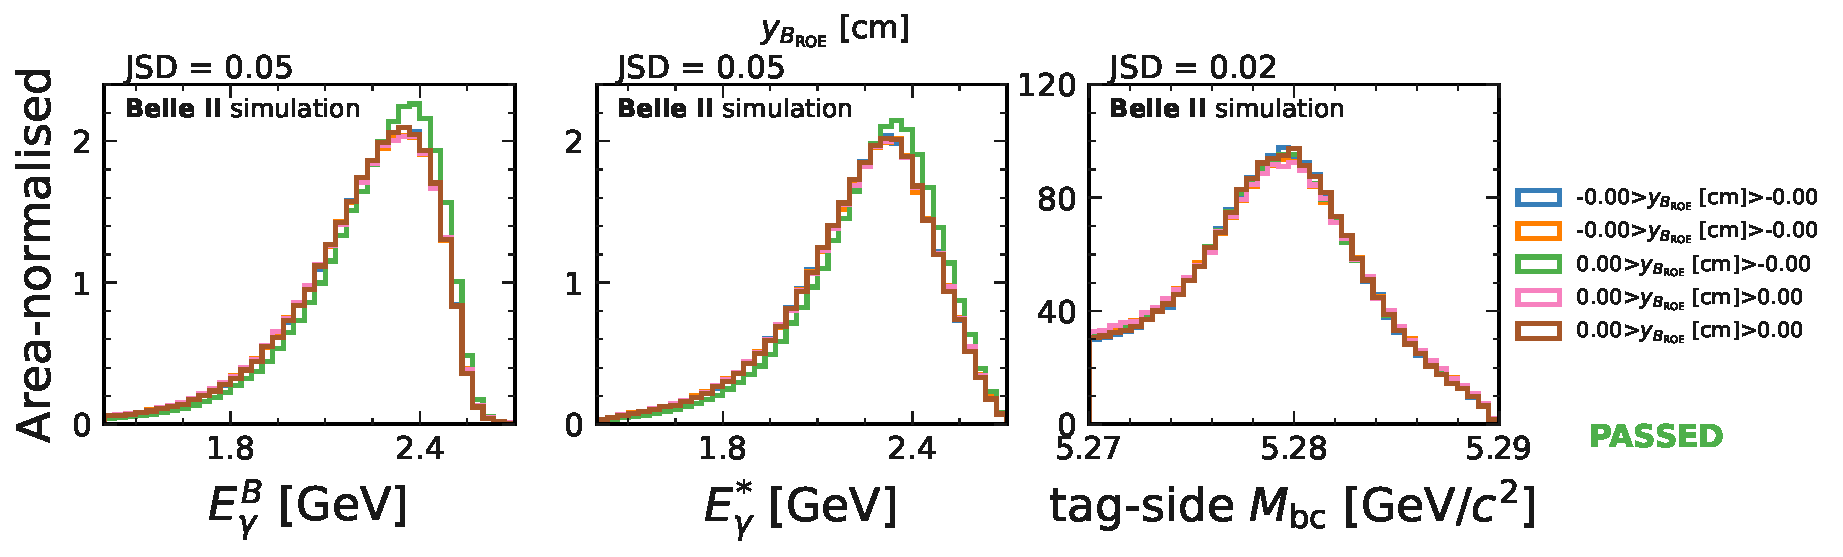
\includegraphics[width=0.95\textwidth]{figures/appendices/continuum_suppression_features/vertex_features/Btag_TagVyBeam_bias_tested.pdf}

    }
    \subcaptionbox{\label{fig:Btag_TagVz}}{
        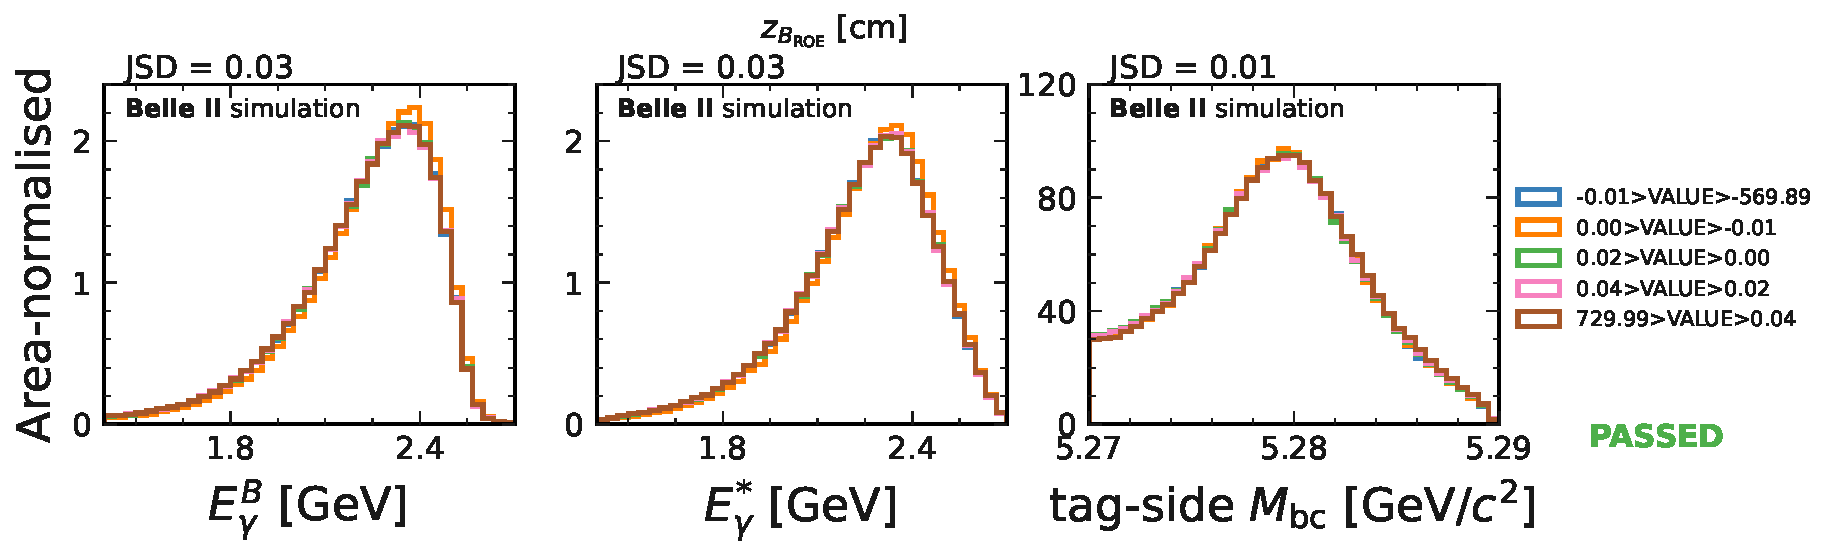
\includegraphics[width=0.95\textwidth]{figures/appendices/continuum_suppression_features/vertex_features/Btag_TagVzBeam_bias_tested.pdf}

    }
    \subcaptionbox{\label{fig:Btag_TagVxErr}}{
        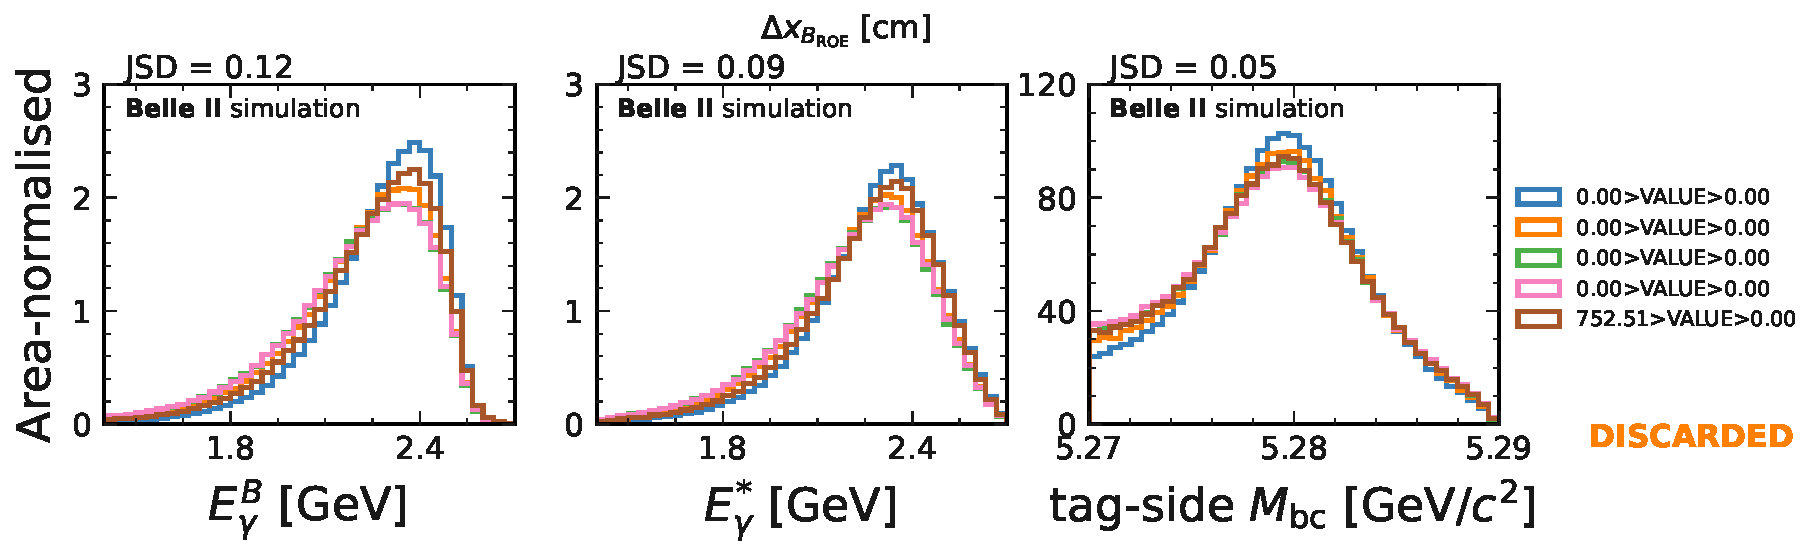
\includegraphics[width=0.95\textwidth]{figures/appendices/continuum_suppression_features/vertex_features/Btag_TagVxErr_bias_tested.pdf}

    }
    \subcaptionbox{\label{fig:Btag_TagVyErr}}{
        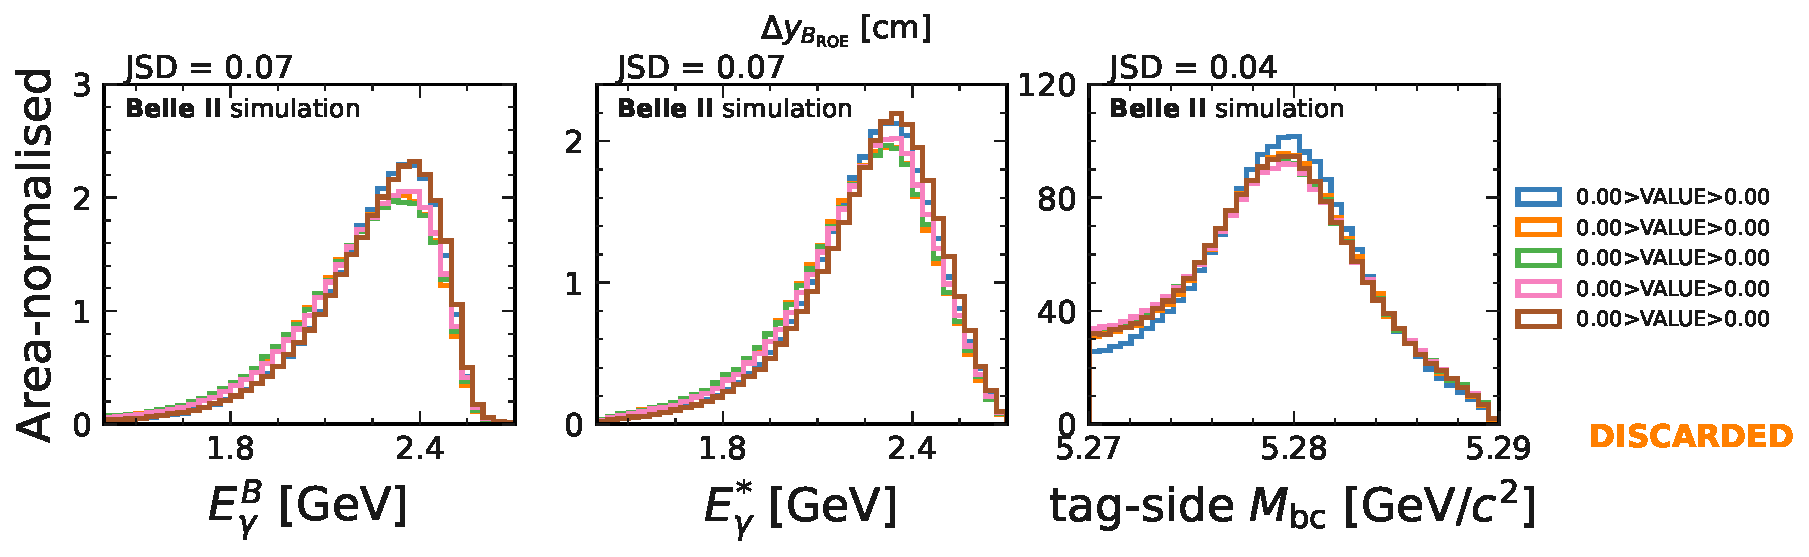
\includegraphics[width=0.95\textwidth]{figures/appendices/continuum_suppression_features/vertex_features/Btag_TagVyErr_bias_tested.pdf}

    }
\end{figure}
\begin{figure}[htbp!]
    \centering
    \ContinuedFloat

    \subcaptionbox{\label{fig:Btag_TagVzErr}}{
        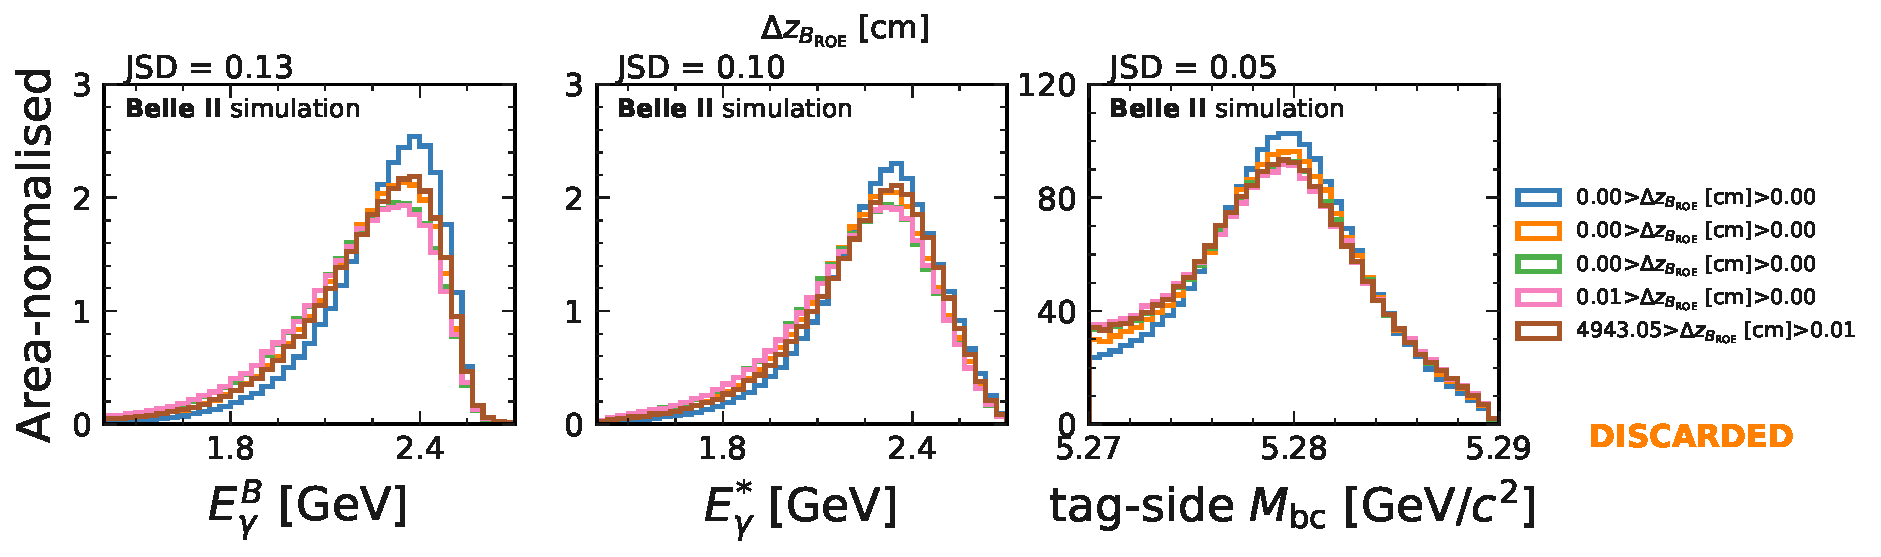
\includegraphics[width=0.95\textwidth]{figures/appendices/continuum_suppression_features/vertex_features/Btag_TagVzErr_bias_tested.pdf}

    }
    \subcaptionbox{\label{fig:Btag_TagVChi2}}{
        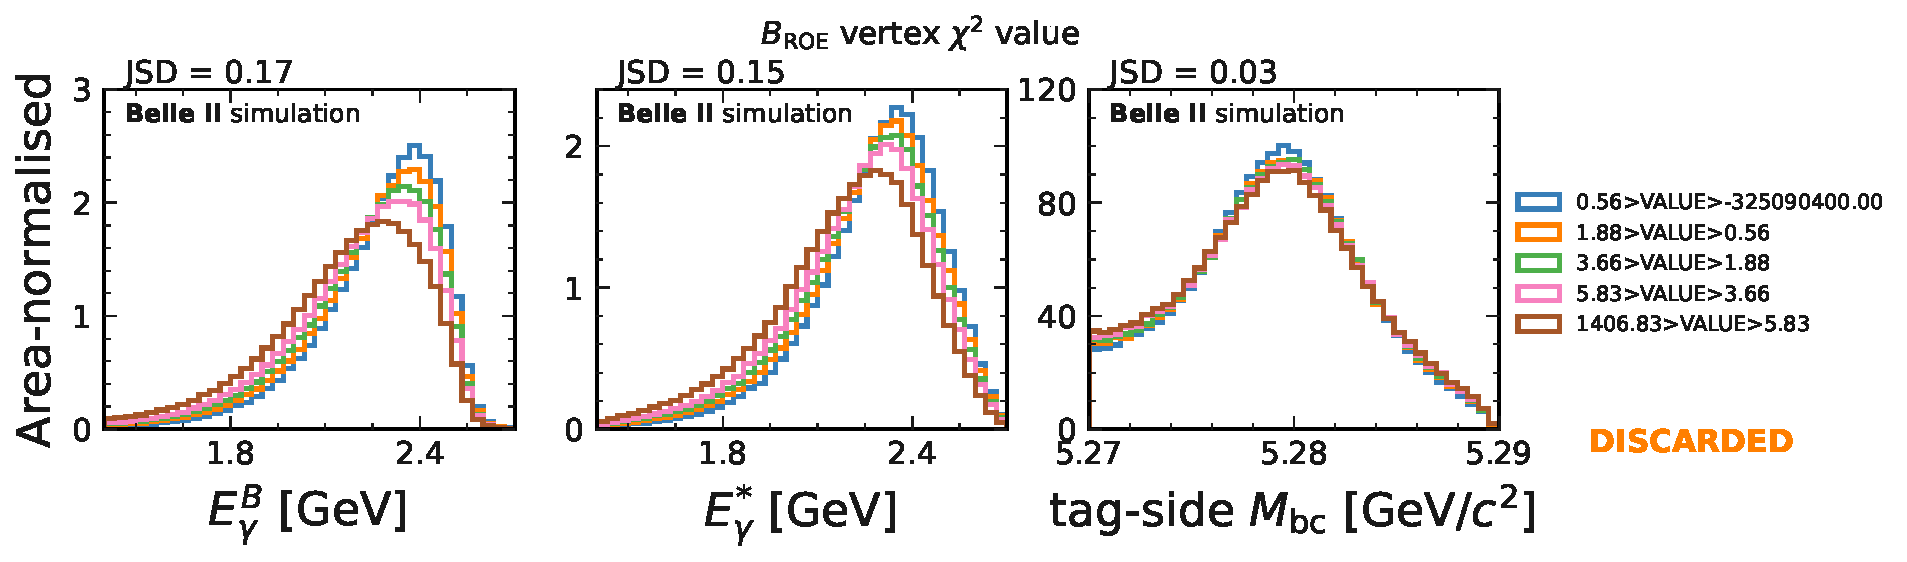
\includegraphics[width=0.95\textwidth]{figures/appendices/continuum_suppression_features/vertex_features/Btag_TagVChi2_bias_tested.pdf}

    }
    \subcaptionbox{\label{fig:Btag_TagVChi2IP}}{
        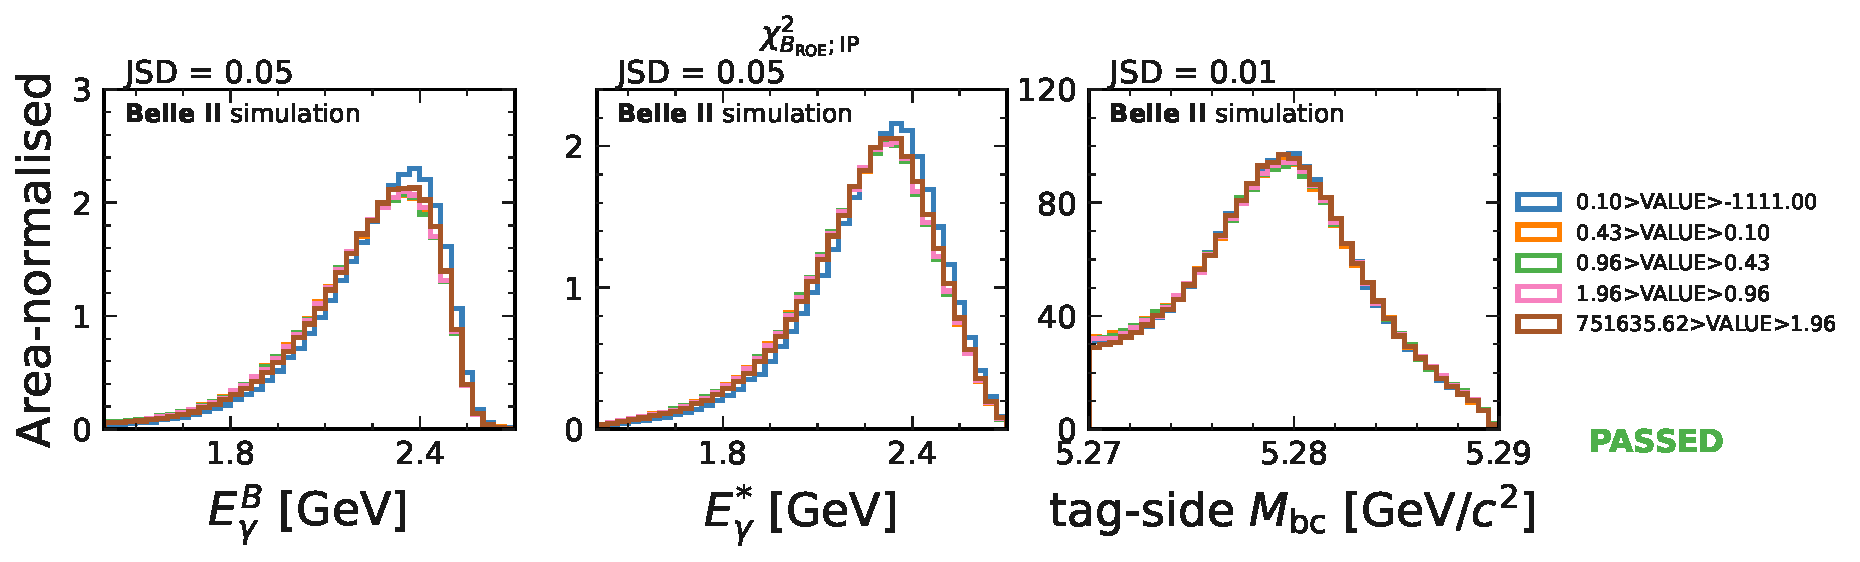
\includegraphics[width=0.95\textwidth]{figures/appendices/continuum_suppression_features/vertex_features/Btag_TagVChi2IP_bias_tested.pdf}

    }
    \subcaptionbox{\label{fig:Btag_TagVpVal}}{
        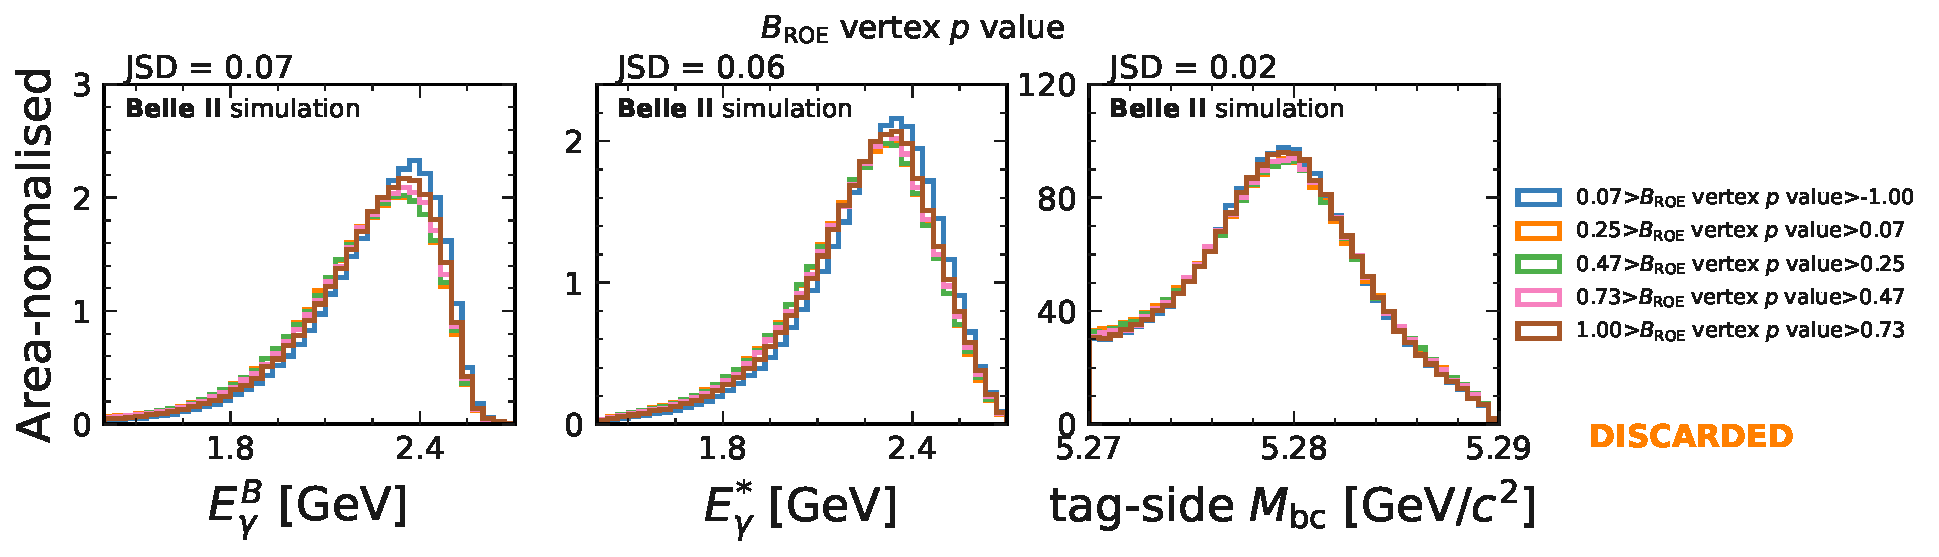
\includegraphics[width=0.95\textwidth]{figures/appendices/continuum_suppression_features/vertex_features/Btag_TagVpVal_bias_tested.pdf}

    }
\end{figure}
\begin{figure}[htbp!]
    \centering
    \ContinuedFloat

    \subcaptionbox{\label{fig:Btag_DeltaT}}{
        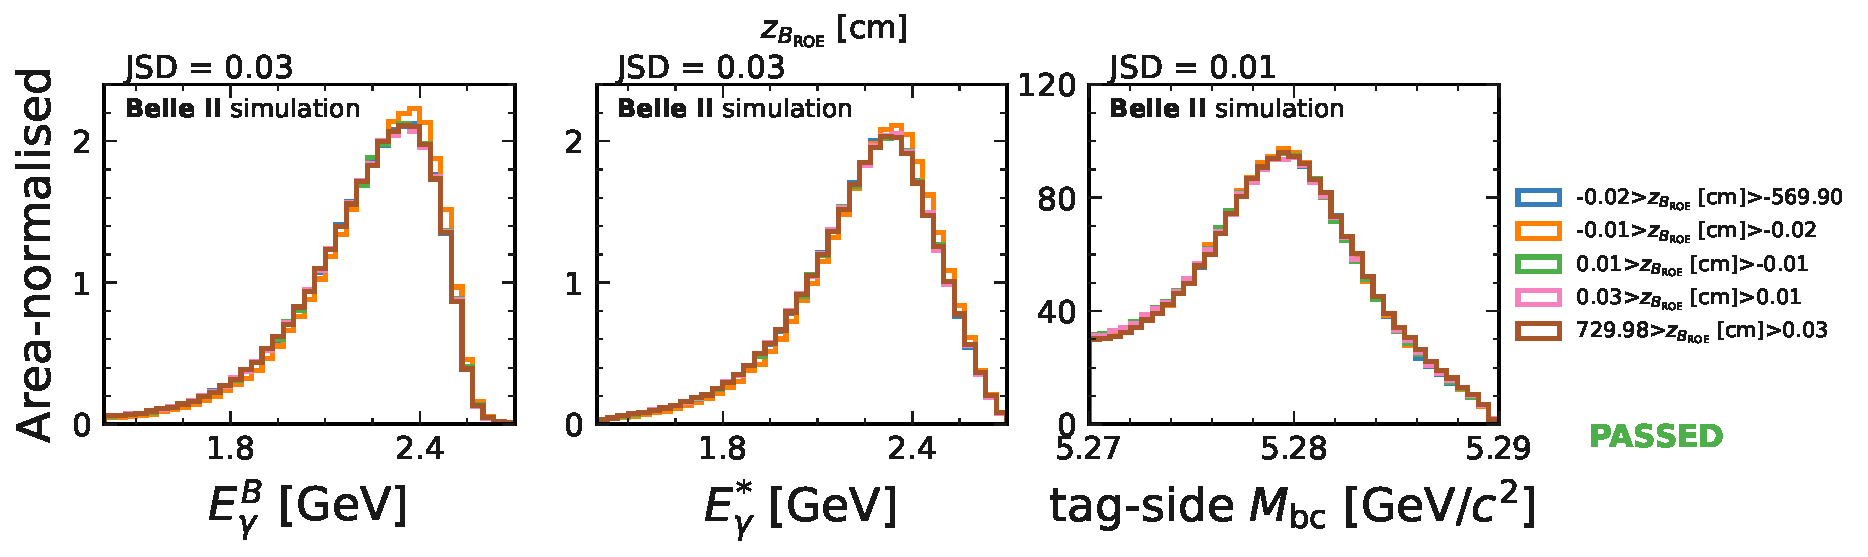
\includegraphics[width=0.95\textwidth]{figures/appendices/continuum_suppression_features/vertex_features/Btag_TagVz_bias_tested.pdf}

    }
    \subcaptionbox{\label{fig:Btag_DeltaZ}}{
        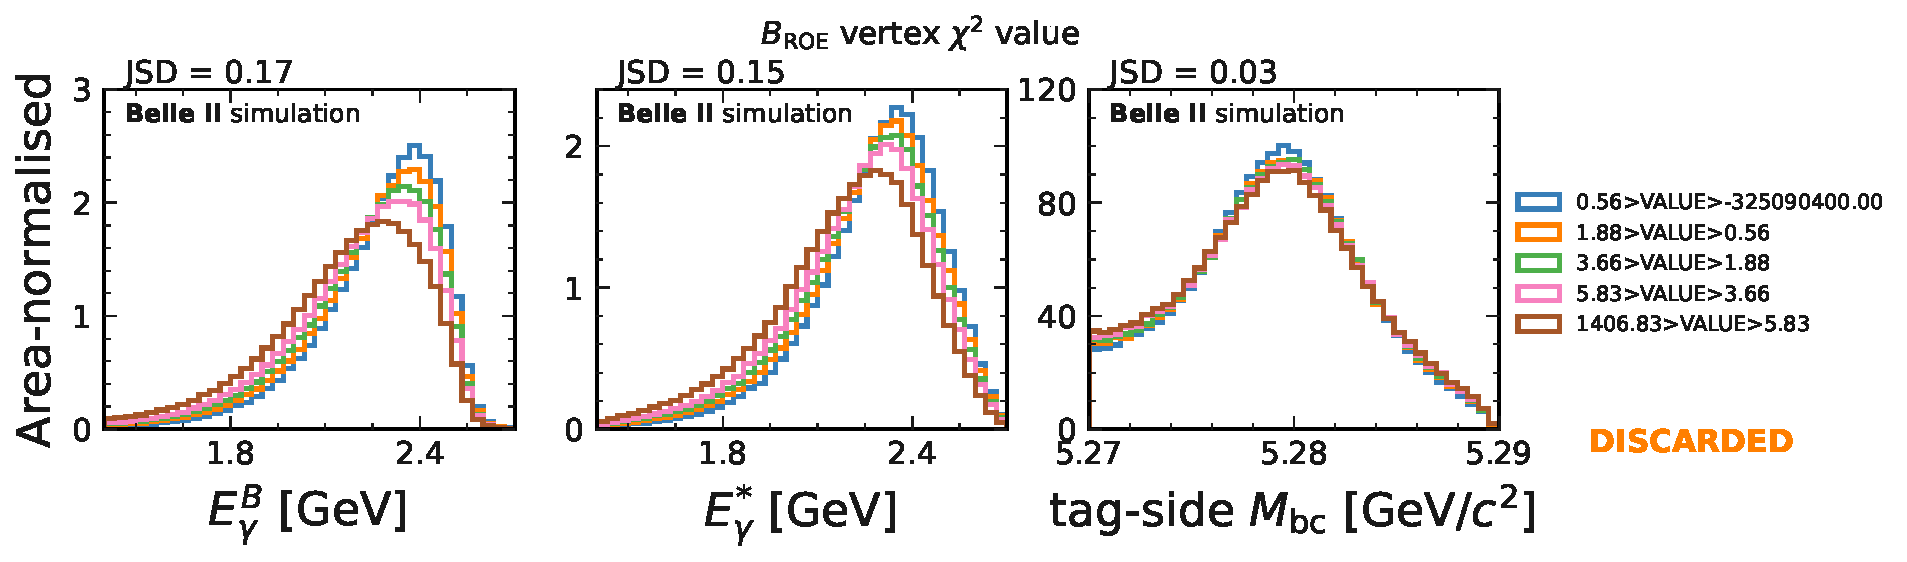
\includegraphics[width=0.95\textwidth]{figures/appendices/continuum_suppression_features/vertex_features/Btag_TagVChi2_bias_tested.pdf}

    }
    \subcaptionbox{\label{fig:Btag_DeltaBoost}}{
        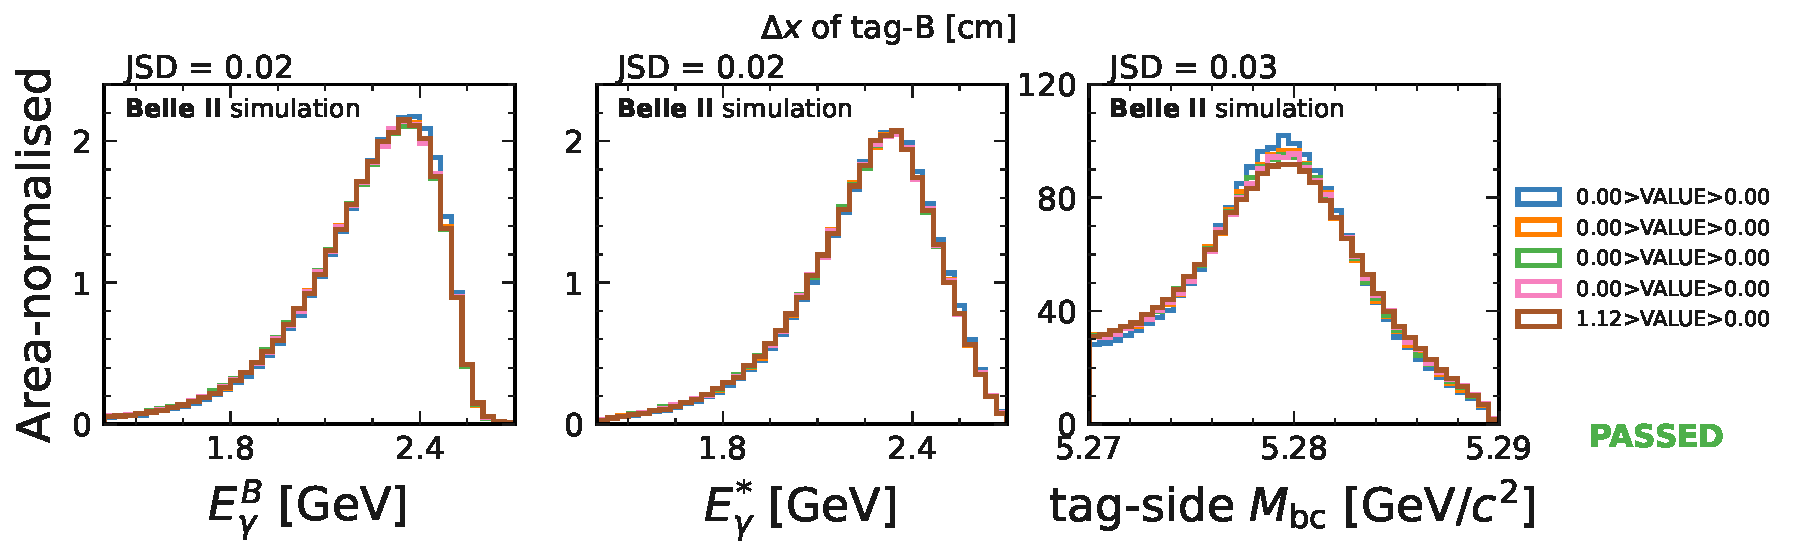
\includegraphics[width=0.95\textwidth]{figures/appendices/continuum_suppression_features/vertex_features/Btag_x_uncertainty_bias_tested.pdf}

    }
    \caption{\label{fig:vertex_features_test1} The bias-test on \EB, \Estar and \Mbc for vertex coordinates of the $B$ mesons.
    The test is performed based on \textbf{Test~1} strategy, defined in \Cref{sec:continuum_features}.
    Variable definitions are given in text.}
\end{figure}